% LaTeX Präsentationsvorlage (2013) der TU Graz, rev12, 2013/01/31
\documentclass{beamer}
% \documentclass[aspectratio=169]{beamer}
% \usetheme{tugraz2013}
% \usetheme[notes]{tugraz2013}
\usetheme{tugraz2013}
\usepackage{caption}
\captionsetup[figure]{labelformat=empty}
\usepackage{color}
\usepackage{multicol}
\usepackage{bbding}
\usepackage{wasysym}

\usepackage{picture}
\usepackage{rotating}

\definecolor{darkred}{rgb}{0.85,0.16,0.0}
\definecolor{darkgreen}{rgb}{0.16,0.70,0.27}

\newcommand{\red}[1]{{\color{red} #1}}
\newcommand{\blue}[1]{{\color{blue} #1}}
\newcommand{\darkgreen}[1]{\textcolor{darkgreen}{#1}}
\newcommand{\darkred}[1]{\textcolor{darkred}{#1}}

\newcommand*{\vpointer}{\vcenter{\hbox{\scalebox{1.5}{\large\pointer}}}}

\newcommand{\be}[1]{\begin{equation} \label{#1}}
\newcommand{\ee}{\end{equation}}
\newcommand{\bea}[1]{\begin{eqnarray} \label{#1}}
\newcommand{\eea}{\end{eqnarray}}
\newcommand{\bean}{\begin{eqnarray*}}
\newcommand{\eean}{\end{eqnarray*}}

\newcommand{\non}{\nonumber\\}
\newcommand{\eq}[1]{(\ref{#1})}
\newcommand{\difp}[2]{\frac{\partial #1}{\partial #2}}
\newcommand{\br}{{\bf r}}
\newcommand{\bR}{{\bf R}}
\newcommand{\bA}{{\bf A}}
\newcommand{\bB}{{\bf B}}
\newcommand{\bE}{{\bf E}}
\newcommand{\bm}{{\bf m}}
%\renewcommand{\bm}{{\bf m}}
\newcommand{\bn}{{\bf n}}
\newcommand{\bN}{{\bf N}}
\newcommand{\bp}{{\bf p}}
\newcommand{\bP}{{\bf P}}
\newcommand{\bF}{{\bf F}}
\newcommand{\by}{{\bf y}}
\newcommand{\bz}{{\bf z}}
\newcommand{\bZ}{{\bf Z}}
\newcommand{\bV}{{\bf V}}
\newcommand{\bv}{{\bf v}}
\newcommand{\bu}{{\bf u}}
\newcommand{\bx}{{\bf x}}
\newcommand{\bX}{{\bf X}}
\newcommand{\bW}{{\bf W}}
\newcommand{\bJ}{{\bf J}}
\newcommand{\bj}{{\bf j}}
\newcommand{\bk}{{\bf k}}
\newcommand{\bTheta}{{\bf \Theta}}
\newcommand{\btheta}{{\boldsymbol\theta}}
\newcommand{\bOmega}{{\bf \Omega}}
\newcommand{\bomega}{{\boldsymbol\omega}}
\newcommand{\brho}{{\boldsymbol\rho}}
\newcommand{\rd}{{\rm d}}
\newcommand{\rJ}{{\rm J}}
\newcommand{\ph}{{\varphi}}
\newcommand{\te}{\theta}
\newcommand{\tht}{\vartheta}
\newcommand{\vpar}{v_\parallel}
\newcommand{\vparkb}{v_{\parallel k b}}
\newcommand{\vparkm}{v_{\parallel k m}}
\newcommand{\Jpar}{J_\parallel}
\newcommand{\ppar}{p_\parallel}
\newcommand{\Bpstar}{B_\parallel^*}
\newcommand{\intpi}{\int\limits_{0}^{2\pi}}
\newcommand{\summ}{\sum \limits_{m=-\infty}^\infty}
\newcommand{\tb}{\tau_b(\uv)}
\newcommand{\bh}{{\bf h}}
\newcommand{\cE}{{\cal E}}
\newcommand{\bsigma}{{\boldsymbol\sigma}}
\newcommand{\bS}{{\mathbf S}}
\newcommand{\bI}{{\mathbf I}}
\newcommand{\odtwo}[2]{\frac{\rd #1}{\rd #2}}
\newcommand{\pdone}[1]{\frac{\partial}{\partial #1}}
\newcommand{\pdtwo}[2]{\frac{\partial #1}{\partial #2}}
\newcommand{\ds}{\displaystyle}

%% Titelblatt-Einstellungen
\title[]
{Geometric Integration of \\Guiding Center Orbits in Magnetically Confined Plasmas and Applications}
\author[L.~Bauer]{\scriptsize Lukas Bauer, BSc. \\
	Institute of Theoretical and Computational Physics - Plasma Physics\\Group of Prof. W. Kernbichler (Graz University of Technology)
}
\date{10. July 2020, Seminar Presentation, Graz} % \today für heutiges Datum verwenden
%\date{\today}
\institute[Institute of Theoretical and Computational Physics]
{
}
\instituteurl{www.tugraz.at}
% \institutelogo{kurz.pdf}
\additionallogo{merged_logos_m.png}

%%%%%%%%%%%%%%%%%%%%%%%%%%%%%%%%%%%%%%%%%%%%%%%%%%%%%%%%%%%%%%%%%%%%%%%%%%%%
\begin{document}
%	\setbeameroption{show notes}% un-comment to see the notes
%%%%%%%%%%%%%%%%%%%%%%%%%%%%%%%%%%%%%%%%%%%%%%%%%%%%%%%%%%%%%%%%%%%%%%%%%%%%
\titleframe

%\begin{frame}
%  \frametitle{Outline}
%  \tableofcontents%[hideallsubsections] 
%  \note{
%  	Meine Präsentation ist wie folgt strukturiert \ldots
%  }
%\end{frame}

%\section{Introduction}
% \begin{frame}
% \begin{center}
% \vfill
% {\Large Motivation}
% \vfill
% \end{center}
% \end{frame}




\section{Introduction to nuclear fusion}

\begin{frame}
	\frametitle{What is nuclear fusion?}
	\vspace{-1 cm}
	\begin{columns}[onlytextwidth]
		\begin{column}{0.45\textwidth}
			\begin{center}
					\begin{figure}
				\includegraphics[trim={0 0 0 2cm},clip,width=0.8\textwidth]{FIGURES/Deuterium-tritium_fusion.png}
				\caption{Deuterium + Tritium \\
					$\rightarrow$ Helium + neutron}
					\end{figure}
			\end{center}
		\end{column}
		\begin{column}{0.45\textwidth}
			\begin{center}
				\begin{itemize}
					\item Two or more atomic nuclei are combined to form one or more different atomic nuclei and subatomic particles\\
					\item 17.6 MeV are released as kinetic energy in the case for D+T fusion\\
				\end{itemize}
			\end{center}
		\end{column}
	\end{columns}
\end{frame}




\begin{frame}
\frametitle{What is the current approach to fusion?}
\vspace{-1.5 cm}
\begin{columns}[onlytextwidth]
	\begin{column}{0.45\textwidth}
		\begin{center}
		\begin{figure}
			
\includegraphics[trim={0 0 0 0cm},clip,width=0.8\textwidth]{FIGURES/Schematic-of-a-Tokamak-fusion-reactor-Source-Fusion-for-energy.eps}
			\caption{Tokamak}
					\includegraphics[trim={0 0 0 0cm},clip,width=0.9\textwidth]{FIGURES/W7X-Spulen_Plasma_blau_gelb.jpg}
		\caption{Stellarator}
		\end{figure}
		\end{center}
	\end{column}
	\begin{column}{0.45\textwidth}
		\vspace{0 cm}
		\begin{center}
			\begin{itemize}
				\item Heating of D-T plasma to $\sim10^7~\text{K}$ in toroidal magnetic configuration
				\item Self sustained reaction according to the Lawson Criterion for the triple product $n\tau T > C$
				\item Two main types of devices: Tokamaks and Stellarators
			\end{itemize}
		\end{center}
	\end{column}
\end{columns}
 \end{frame}

\begin{frame}
\frametitle{Theoretical descriptions of plasmas}
\vspace{-1.5 cm}
\begin{columns}[onlytextwidth]
	\begin{column}{0.5\textwidth}
		\begin{center}
			\begin{itemize}
			\item Magnetohydro-\\
			dynamics (MHD)
			\begin{itemize}
				\item describes the plasma as an electrically conducting fluid
				\item only valid at high particle collisionalities \\
				$\rightarrow$ velocity distributions are considered to be Maxwellian
			\end{itemize}
			\end{itemize}
		\end{center}
	\end{column}
	\begin{column}{0.5\textwidth}
		\begin{center}
			\begin{itemize}
			\item Kinetic Approach
				\begin{itemize}
						\item description of plasma through discrete particle distribution functions $f(\vec{x},\vec{v})$ of phase space
						\item coupling Vlasov + Maxwells equations
				\end{itemize}
			\item Gyro-kinetic Approach
				\begin{itemize}
				\item averaging over gyrating motion around field lines
				\item reduced distribution function $f(\vec{x},v_\parallel, v_\perp)$
			\end{itemize}
			\end{itemize}
		\end{center}
	\end{column}
\end{columns}
 \end{frame}

\begin{frame}
\frametitle{Guiding center motion}
\vspace{-1 cm}
\begin{columns}[onlytextwidth]
	\begin{column}{0.45\textwidth}
		\begin{center}
		\begin{figure}
					\includegraphics[trim={0 2cm 0cm 0cm},clip,width=1.1\textwidth]{FIGURES/guiding_center.jpg}
\caption{Guiding center motion}	
\end{figure}
		\end{center}
	\end{column}
	\begin{column}{0.45\textwidth}
		\begin{center}
			\begin{itemize}
				\item particles gyrate around field lines
				\item $\rightarrow$ average over fast gyration
				\item corrections to motion in form of drifts
				\item for gyro-kinetic approach many particles need to be traced in boxes
			\end{itemize}
		\end{center}
	\end{column}
\end{columns}
\end{frame}


\section{Introduction to \texttt{Gorilla}}
%\sectionheader[M. Eder, C.G. Albert, S.V. Kasilov, W. Kernbichler]{Three-dimensional geometric integrator for charged particle orbits in toroidal fusion devices}

\begin{frame}
\frametitle{\textbf{Gorilla} guiding center code}
\begin{columns}[onlytextwidth]
	\begin{column}{0.5\textwidth}

		\begin{center}
	\includegraphics[trim={5cm 13cm 1cm 4cm},clip,width=1\textwidth]{FIGURES/guiding_center_drawn2.pdf}
\end{center}
\end{column}
	\begin{column}{0.50\textwidth}
			\begin{center}
	\begin{itemize}
		\item \textbf{G}eometric \textbf{OR}bit \textbf{I}ntegration with \textbf{L}ocal \textbf{L}inearisation \textbf{A}pproach
		\item Integration of charged particle guiding center orbits in toroidal fusion devices
	\end{itemize}
\end{center}
	\end{column}
	\end{columns}
\end{frame}


\begin{frame}
\frametitle{Target application - kinetic equilibria}
\begin{itemize}
\item Kinetic modelling of edge plasmas
\item Quasi-steady plasma parameters in 3D toroidal fusion devices
\begin{itemize}
\item Simple (cylindrical) modelling of perturbed tokamak equilibria shows that the problem of shielding of external perturbations is essentially kinetic.
\item 3D equilibria should be computed by using plasma response currents and charges in kinetic approximation. \\
$\rightarrow$ Global Monte Carlo modelling
\end{itemize}
\end{itemize}
\end{frame}




\begin{frame}
\frametitle{Modelling of kinetic equilibria}
%\vspace{-1.5cm}
	\centering \includegraphics[trim={0 0 0 3cm},clip,width=\textwidth]{FIGURES/cycle01.pdf}
\end{frame}


%\begin{frame}[noframenumbering]
%\frametitle{Modelling of kinetic equilibria}
%%\vspace{-1.5cm}
%	\centering \includegraphics[trim={0 0 0 3cm},clip,width=\textwidth]{FIGURES/cycle02.pdf}
%\end{frame}






\begin{frame}
\frametitle{Requirements to orbit integrator}
\vspace{-0.5cm}
\begin{enumerate}
\item \textbf{Physically correct long time orbit dynamics}
\item \textbf{Low sensitivity to noise in fields:} Perturbation field from plasma response currents and charges is noisy due to stochasticity of particle collisions (Monte Carlo).
\item \textbf{Integrator efficiency:} Millions of orbits should be followed for few collision times at each iteration.
\item \textbf{Efficient box counting:} Orbit intersections with boundaries of grid cells should be traced efficiently.

\end{enumerate}
\end{frame}

%\section{3D Geometric Integrator}

\begin{frame}
\frametitle{\textbf{Gorilla} 3D geometric integrator properties}
\vspace{-0.5cm}
\begin{itemize}
	\item \textbf{Physically correct long time orbit dynamics}
	\begin{itemize}
		\item preserved total energy
		\item preserved magnetic moment
		\item preserved phase space volume 
	\end{itemize}
	\item \textbf{Computationally efficient:} Relaxed requirements to the accuracy of guiding center orbits
		\begin{itemize}
			\item not exact orbit shape
			\item not exact time evolution
		\end{itemize}
\end{itemize}
\end{frame}

\begin{frame}
\frametitle{Formulation of the geometric integrator}
\note{Guiding center equations!! Talk about linearizations, explain that we have 4 independent phasespace variables}
\vspace{-0.5cm}
Use the Hamiltonian form of guiding center equations in curvilinear coordinates,
\be{eqm_curv}
\dot x^i = \frac{v_\parallel \varepsilon^{ijk}}{\sqrt{g} B_\parallel^\ast}\difp{A^\ast_k}{x^j}, \qquad A^\ast_k = A_k + \frac{v_\parallel}{\omega_c}B_k,
\ee
\be{}
v_\parallel=\sigma \left(\frac{2}{m_\alpha}\left(w-J_\perp\omega_c-e_\alpha\Phi\right)\right)^{1/2}.
\ee
\vspace{0.2cm}\\
Approximate $A_k, B_k/ \omega_c$, $\omega_c$ and $\Phi$ by linear functions in spatial cells with equations of motion
\be{standeqset}
\frac{\rd z^i}{\rd \tau} = a^i_k z^k + b^i.
\ee
\end{frame}


\begin{frame}
\frametitle{Physically correct long time orbit dynamics}
\vspace{-0.5cm}
\begin{itemize}
	\item
	Linear approximation of field quantities does \textbf{not destroy the Hamiltonian nature} of the original guiding center equations.
	\item Non-canonical Hamiltonian form of linear ODE set
	\be{hamform}
	\frac{\rd z^i}{\rd \tau}=\Lambda^{ij}\difp{H}{z^j}, \qquad \Lambda^{ij}(\bz)=\left\{z^i,z^j\right\}_\tau,
	\ee
	with Hamiltonian $H(\bz)=v_\parallel^2/2-U(\bx)$ and antisymmetric Poisson matrix  $\Lambda^{ij}(\bz)$.
	\item \textbf{Symplecticity:} Phase space volume is conserved.
\end{itemize}

\end{frame}

\section{Implementation of the grid}

\begin{frame}
\frametitle{Grid for \textbf{Gorilla}}
\begin{itemize}
\item Grid necessary for calculations due to
\begin{itemize}
\item linearization of field quantities
\item box counting scheme for distribution function
\end{itemize}
 $\rightarrow$ guiding center orbits are computed between cell boundaries using a standard $RK4$-integrator
\end{itemize}
\end{frame}


%\begin{frame}
%\frametitle{Global Monte Carlo modelling}
%\begin{itemize}
%\item The purpose is integration of guiding center orbits for Monte Carlo evaluation of plasma response to external non-axisymmetric perturbations from ELM mitigation coils. 
%\item Namely, this is the perturbed pressure tensor, parallel current and charge density needed for iterative solution of Maxwell equations within kinetic modelling of plasma equilibrium.
%\end{itemize}
%\end{frame}

\section{Requirements to the grid}
\begin{frame}
\frametitle{Requirements to grid: Tetrahedral cells}
\begin{itemize}
	\item linear system of equations for $\nabla f = const.$
 \begin{equation}
		\nonumber
		f(\vec{x}_i) = f(\vec{x}_1) + \left(\vec{x}_i-\vec{x}_1\right)\cdot \nabla f, ~i \in \{1,2,3,4\}
	\end{equation}
	\item this system is uniquely defined as the number of unknowns (=4) is equal to the number of values for f\\
	 $\rightarrow$ no fitting for the case of tetrahedra
\end{itemize}
\end{frame}

\begin{frame}
\frametitle{Linearization leads to continuous $f$}
\begin{columns}[onlytextwidth]
	\begin{column}{0.45\textwidth}
		\begin{center}
		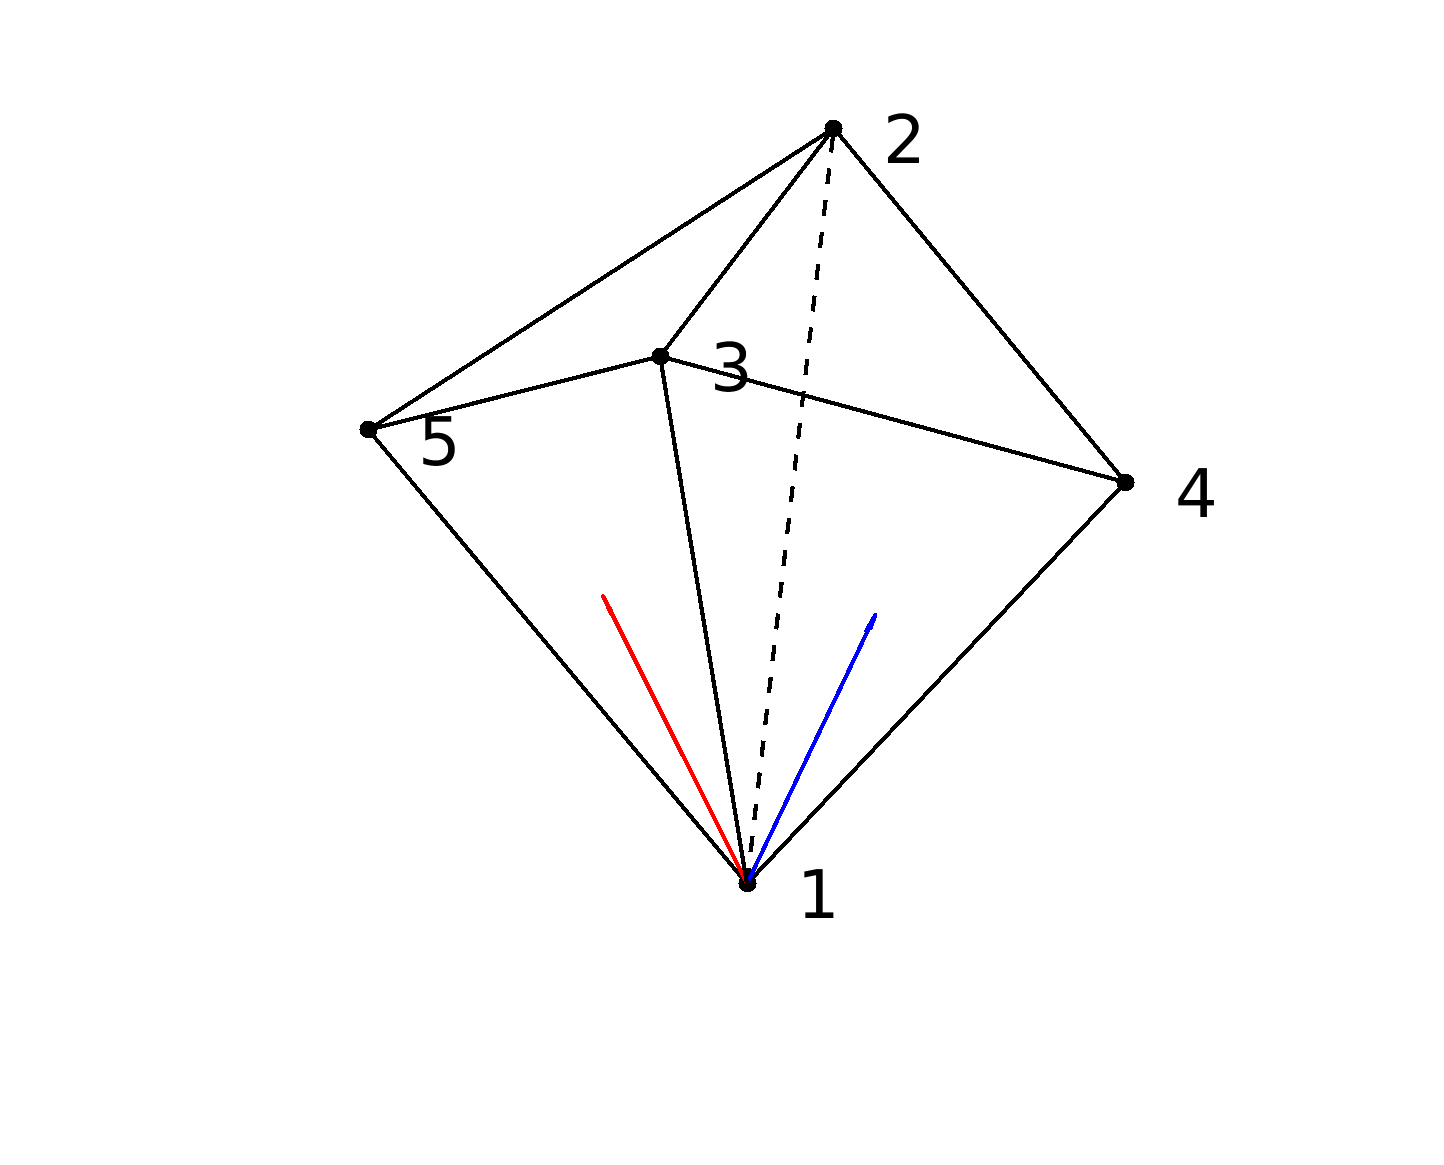
\includegraphics[trim={0 0 0 0.5cm},clip,width=1\textwidth]{FIGURES/linearization.eps}
	\end{center}
	\end{column}
	\begin{column}{0.55\textwidth}
		\begin{center}
		\begin{itemize}
			\item influence of points \{4,5\} vanishes on the plane spanned by \{1,2,3\}\\
			$\rightarrow$ $f$ is continuous at cell boundaries
			\item but: piece-wise constant gradients remain discontinuous at cell boundaries
		\end{itemize}
	\end{center}
\end{column}
\end{columns}
\end{frame}


\begin{frame}
\frametitle{No hanging nodes}
\begin{columns}[onlytextwidth]
	\begin{column}{0.45\textwidth}
		\begin{center}
\centering \includegraphics[trim={4 0 0 0.5cm},clip,width=1\textwidth]{FIGURES/HangingNode.eps}
\end{center}
\end{column}
	\begin{column}{0.55\textwidth}
	\begin{center}
				\begin{itemize}
			\item adjacent tetrahedral faces must share three common vertices for linearized fields to be continuous\\
			$\rightarrow$ no hanging nodes!
		\end{itemize}
	\end{center}
\end{column}
\end{columns}
\end{frame}

\begin{frame}
\frametitle{Further requirements}
\begin{itemize}
	\item whole domain must be unambiguously covered by tetrahedra $\rightarrow$ no holes or overlaps in grid
	\item tetrahedra must be uniquely indexed, also the corresponding neighboring tetrahedra and the faces through which they are connected
	\item periodic boundaries must be taken into account due to coordinate jump
\end{itemize}
\end{frame}

\section{Cylindrical contour grid}
\begin{frame}
\frametitle{Initial grid: cylindrical contour grid}
\vspace{-1.5 cm}
\begin{columns}[onlytextwidth]
	\begin{column}{0.45\textwidth}
		\begin{center}
			\begin{figure}
				\includegraphics[trim={0 1cm 0 2cm},clip,width=0.8\textwidth]{FIGURES/3d_grid_sketch_torus.pdf}
				\caption{Hexahedra}
				\includegraphics[trim={0 3cm 0cm 2cm},clip,width=0.8\textwidth]{FIGURES/Tetra_split.eps}
				\caption{Tetrahedra}
			\end{figure}
		\end{center}
	\end{column}
	\begin{column}{0.45\textwidth}
		\vspace{0 cm}
		\begin{center}
			\begin{itemize}
				\item vertices lie on contours of cylindrical coordinates $(R,\varphi,Z)$
				\item hexahedra are obtained by indexing vertices
				\item each hexahedron is cut into six tetrahedra
				\item neighboring tetrahedra need to be indexed for logics
			\end{itemize}
		\end{center}
	\end{column}
\end{columns}
\end{frame}

\begin{frame}
\frametitle{Cylindrical contour grid}
\vspace{-1 cm}
\begin{columns}[onlytextwidth]
	\begin{column}{0.5\textwidth}
		\begin{center}
			\begin{figure}
				\includegraphics[trim={0 1cm 0 3cm},clip,width=1\textwidth]{FIGURES/slice_grid_rect.png}
				\caption{toroidal grid slice}
			\end{figure}
		\end{center}
	\end{column}
	\begin{column}{0.5\textwidth}
		\vspace{1.25 cm}
		\begin{center}
	\begin{figure}
		\includegraphics[trim={0 1cm 0 2cm},clip,width=1\textwidth]{FIGURES/full_grid_rect.png}
		\caption{full cylindrical contour grid}
	\end{figure}
\end{center}
	\end{column}
\end{columns}
\end{frame}

\begin{frame}
\frametitle{Poincaré plots of guiding center orbits}
\vspace{-0.75 cm}
\begin{columns}[onlytextwidth]
	\begin{column}{0.55\textwidth}
		\begin{center}
			\begin{figure}
				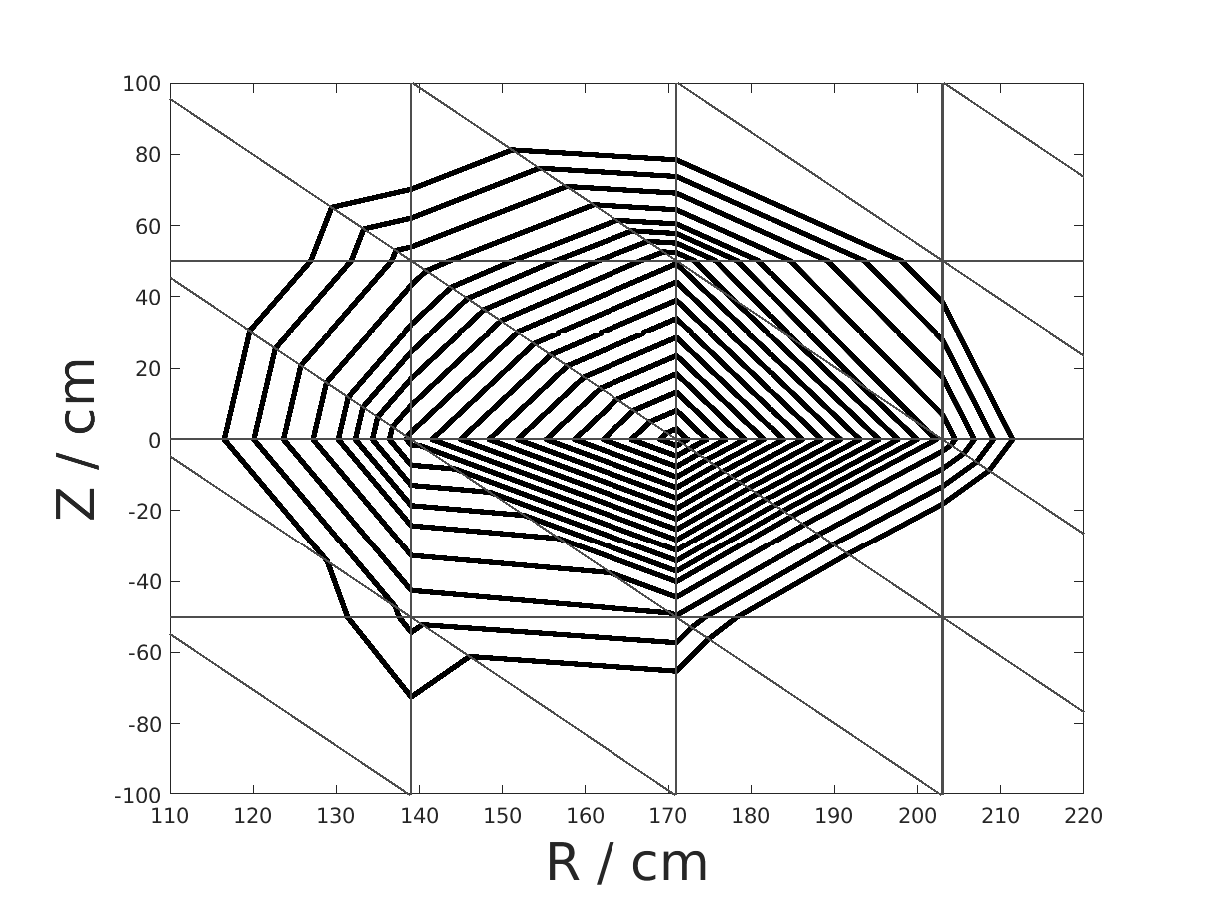
\includegraphics[trim={0cm 0cm 0cm 0cm},clip,width=1\textwidth]{FIGURES/field_lines_rect_grid2.eps}
				\caption{}
			\end{figure}
		\end{center}
	\end{column}
	\begin{column}{0.45\textwidth}
		\vspace{0 cm}
		\begin{center}
			\begin{itemize}
				\item intersections of orbits with $\varphi=0$ plane are marked with points
				\item points lie on well-defined contours
				\item polygonal shape due to linearization 
			\end{itemize}
		\end{center}
	\end{column}
\end{columns}
\end{frame}



\section{Symmetry flux coordinates}
\begin{frame}
\frametitle{Idea: symmetry flux coordinates}
\vspace{-1 cm}
\begin{columns}[onlytextwidth]
	\begin{column}{0.5\textwidth}
		\begin{center}
			\begin{figure}
				\includegraphics[trim={0 0cm 0 0cm},clip,width=1\textwidth]{FIGURES/magnetic_field_labeled0.jpg}
				\caption{Magnetic field topology}
			\end{figure}
		\end{center}
	\end{column}
	\begin{column}{0.5\textwidth}
		\vspace{0 cm}
		\begin{center}
			\begin{itemize}
				\item coordinates $(s,\vartheta,\varphi)$\\
							\begin{itemize}
					\item $s\rightarrow$ minor-radial coordinate
					\item $\vartheta \rightarrow$ poloidal coordinate
					\item $\varphi \rightarrow$ toroidal coordinate
				\end{itemize}
				\item field lines assume straight lines in SFC
				\item $\vec{A}\propto s$
				$\rightarrow$ no interpolation error due to linearization
			\end{itemize}
		\end{center}
	\end{column}
\end{columns}
\end{frame}

\begin{frame}[noframenumbering]
\frametitle{Idea: symmetry flux coordinates}
\vspace{-1 cm}
\begin{columns}[onlytextwidth]
	\begin{column}{0.5\textwidth}
	
		\begin{center}
			\begin{figure}
				\includegraphics[trim={0 0cm 0 0cm},clip,width=1\textwidth]{FIGURES/magnetic_field_labeled0.jpg}
				\caption{Magnetic field topology}
			\end{figure}
		\end{center}
	\end{column}
	\begin{column}{0.5\textwidth}
		\vspace{0 cm}
		\begin{center}
			\begin{itemize}
				\item coordinates $(s,\vartheta,\varphi)$\\
				\begin{itemize}
					\item $s\rightarrow$ minor-radial coordinate
					\item $\vartheta \rightarrow$ poloidal coordinate
					\item $\varphi \rightarrow$ toroidal coordinate
				\end{itemize}
				\item field lines assume straight lines in SFC
				\item $\vec{A}\propto s$
				$\rightarrow$ no interpolation error due to linearization
			\end{itemize}
		\end{center}
	\end{column}
\end{columns}
\vspace{0.4 cm}
\textbf{Problem with CCG: incompatible with SFC}
\end{frame}

\section{Field aligned grid}
\begin{frame}
\frametitle{Implementing a field aligned grid}
\vspace{-1 cm}
\begin{columns}[onlytextwidth]
	\begin{column}{0.5\textwidth}
		\begin{center}
			\begin{figure}
				\includegraphics[trim={0 0cm 0 0cm},clip,width=1\textwidth]{FIGURES/magnetic_field_labeled.jpg}
\caption{Magnetic field topology}
			\end{figure}
		\end{center}
	\end{column}
	\begin{column}{0.5\textwidth}
		\vspace{0 cm}
		\begin{center}
			\begin{itemize}

				\item find $O$-point and $X$-point
				\item field line integration for coordinate interpolation
				\item interpolation routine: $(s,\vartheta,\varphi)\rightarrow (R,\varphi,Z)$ for evaluation of field quantities
				\item create 2D grid points \newline $\rightarrow$ extrude to 3D
				\item connect vertices to form tetrahedra
			\end{itemize}
		\end{center}
	\end{column}
\end{columns}
\end{frame}


\begin{frame}
\frametitle{Field-line integration}
\vspace{-0.5 cm}
\begin{columns}[onlytextwidth]
	\begin{column}{0.5\textwidth}
		\begin{center}
			\begin{figure}
				\includegraphics[trim={0 0cm 0 0cm},clip,width=1\textwidth]{FIGURES/field_lines_torus.pdf}
				\caption{Selected field lines in torus}
			\end{figure}
		\end{center}
	\end{column}
	\begin{column}{0.5\textwidth}
		\vspace{0 cm}
		\begin{center}
			\begin{itemize}
				\item Field line equations: $\frac{\textrm{d}R}{\textrm{d}\varphi} = \frac{B^R}{B^\varphi}, \hspace{0.1cm} \frac{\textrm{d}Z}{\textrm{d}\varphi} = \frac{B^Z}{B^\varphi}
				$
				\vspace{1cm}
				\item Safety factor: \newline $q_s = \frac{B^\varphi}{B^\vartheta},~\textrm{d}\varphi= q_s\textrm{d}\vartheta
				$
					\begin{itemize}
					\item if $q_s$ is irrational, the field line forms a flux surface
				\end{itemize}
			\end{itemize}
		\end{center}
	\end{column}
\end{columns}
\end{frame}



\begin{frame}
\frametitle{Finding the $O$-point}
\vspace{-1 cm}
\begin{columns}[onlytextwidth]
	\begin{column}{0.5\textwidth}
		\begin{center}
			\begin{figure}
				\includegraphics[trim={6cm 5cm 1.5cm 5cm cm},clip,width=0.6\textwidth]{FIGURES/getOpoint.pdf}
				\caption{Iterative scheme for finding the $O-point$}
			\end{figure}
		\end{center}
	\end{column}
	\begin{column}{0.5\textwidth}
		\vspace{0 cm}
		\begin{center}
			\begin{itemize}
				\item start at point $1$, follow $\vec{B}$ for 10 toroidal turns in $(R,\varphi,Z)$
				\item  compute average of $(R,Z)\rightarrow$ new starting point for the next iteration
				\item perform 20 iterations for satisfying accuracy of the magnetic axis
			\end{itemize}
		\end{center}
	\end{column}
\end{columns}
\end{frame}

\begin{frame}
\frametitle{Finding the $X$-point}
\vspace{-1 cm}
\begin{columns}[onlytextwidth]
	\begin{column}{0.5\textwidth}
		\begin{center}
			\begin{figure}
				\includegraphics[trim={6cm 2.5cm 1.5cm 5cm cm},clip,width=0.6\textwidth]{FIGURES/getXpoint.pdf}
				\caption{Iterative scheme for finding the $X-point$}
			\end{figure}
		\end{center}
	\end{column}
	\begin{column}{0.5\textwidth}
		\vspace{0 cm}
		\begin{center}
			\begin{itemize}
				\item start inside and integrate field line for one poloidal turn
				\item increase distance to mag. axis and repeat until the field line does not cross $\rightarrow$ Separatrix
				\item perform iterative integrations with $\Delta\varphi= 2\pi/10$
				$\rightarrow$ convergence, since $B^{pol} = 0$ at $X$-point
			\end{itemize}
		\end{center}
	\end{column}
\end{columns}
\end{frame}

\begin{frame}
\frametitle{Massive computation of field lines}
\vspace{0 cm}
%\begin{columns}[onlytextwidth]
%	\begin{column}{0.5\textwidth}
%		\begin{center}
%			\begin{figure}
%				\includegraphics[trim={0 0cm 0 0cm},clip,width=1\textwidth]{FIGURES/}
%				\caption{}
%			\end{figure}
%		\end{center}
%	\end{column}
%	\begin{column}{0.5\textwidth}
		\vspace{-0.5 cm}
		\begin{center}
			\begin{itemize}
				\item parametrize line segment from $O$-point to $X$-point with 500 equidistant starting points $\rightarrow$ $\vartheta=0$-contour
				\item integrate each line for one poloidal turn $\rightarrow$ compute $q_s$
				\item integrate each line for one poloidal turn over 500 equidistant steps $\rightarrow$ save $(R,Z)$ together with poloidal and normalized toroidal flux $s$ and poloidal angle $\vartheta = i/500$ with current step $i$
				\item due to axisymmetry $\varphi$ is equal to the cyl. coordinates toroidal angle
			\end{itemize}
		\end{center}
%	\end{column}
%\end{columns}
\end{frame}

\begin{frame}
\frametitle{Interpolation of $(R,Z)$ from $(s,\vartheta)$}
\vspace{0 cm}
%\begin{columns}[onlytextwidth]
%	\begin{column}{0.5\textwidth}
%		\begin{center}
%			\begin{figure}
%				\includegraphics[trim={0 0cm 0 0cm},clip,width=1\textwidth]{FIGURES/}
%				\caption{}
%			\end{figure}
%		\end{center}
%	\end{column}
%	\begin{column}{0.5\textwidth}
		\vspace{0 cm}
		\begin{center}
			\begin{itemize}
				\item compute periodic spline coefficients in $\vartheta$ for each saved field line, $s=const.$ along a field line
				\item for a given value of $\vartheta$, evaluate interpolated values of $R,Z$ for field lines which are adjacent to $s$
				\item use Lagrange polynomial interpolation to compute $R(s,\vartheta),~ Z(s,\vartheta)$ 
			\end{itemize}
		\end{center}
%	\end{column}
%\end{columns}
\end{frame}

\begin{frame}
\frametitle{Lagrange polynomial interpolation}
\vspace{-1.5cm}
\begin{columns}[onlytextwidth]
	\begin{column}{0.5\textwidth}
		\begin{center}
			\begin{figure}
				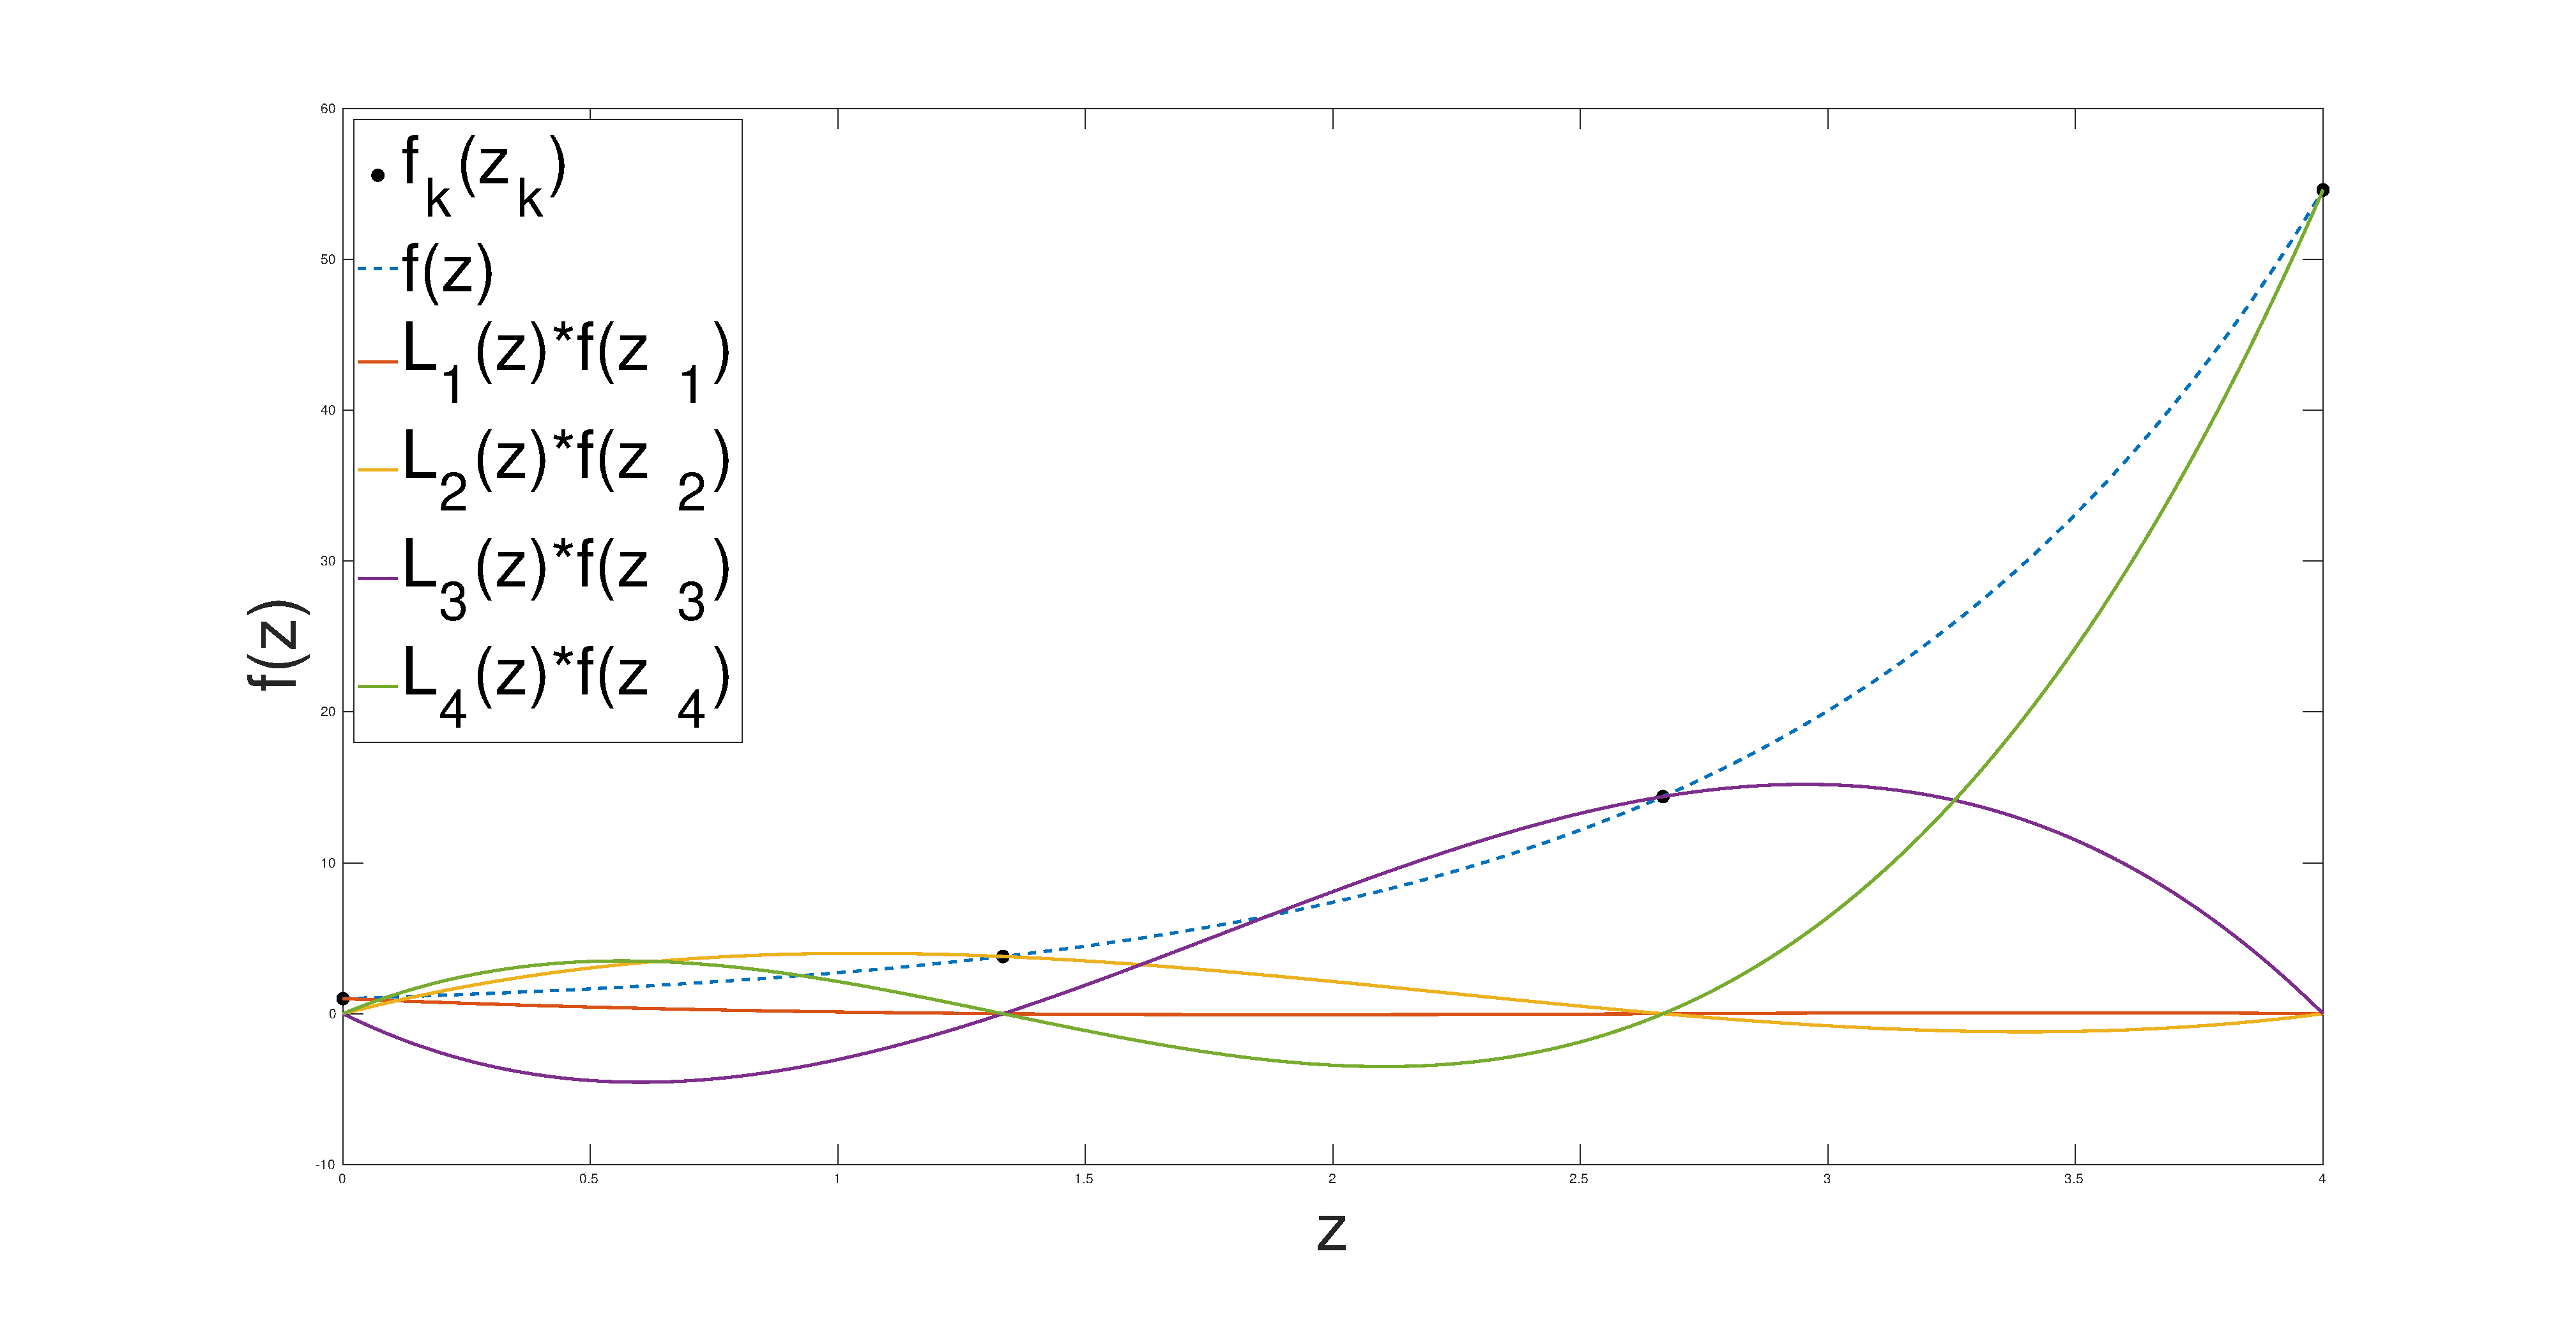
\includegraphics[trim={0 0cm 0 0cm},clip,width=1\textwidth]{FIGURES/lag_interp_plot1.eps}
					\vspace{-0.5cm}
					\caption{Depiction of $L_k(z)$}
										\vspace{-0.35cm}
				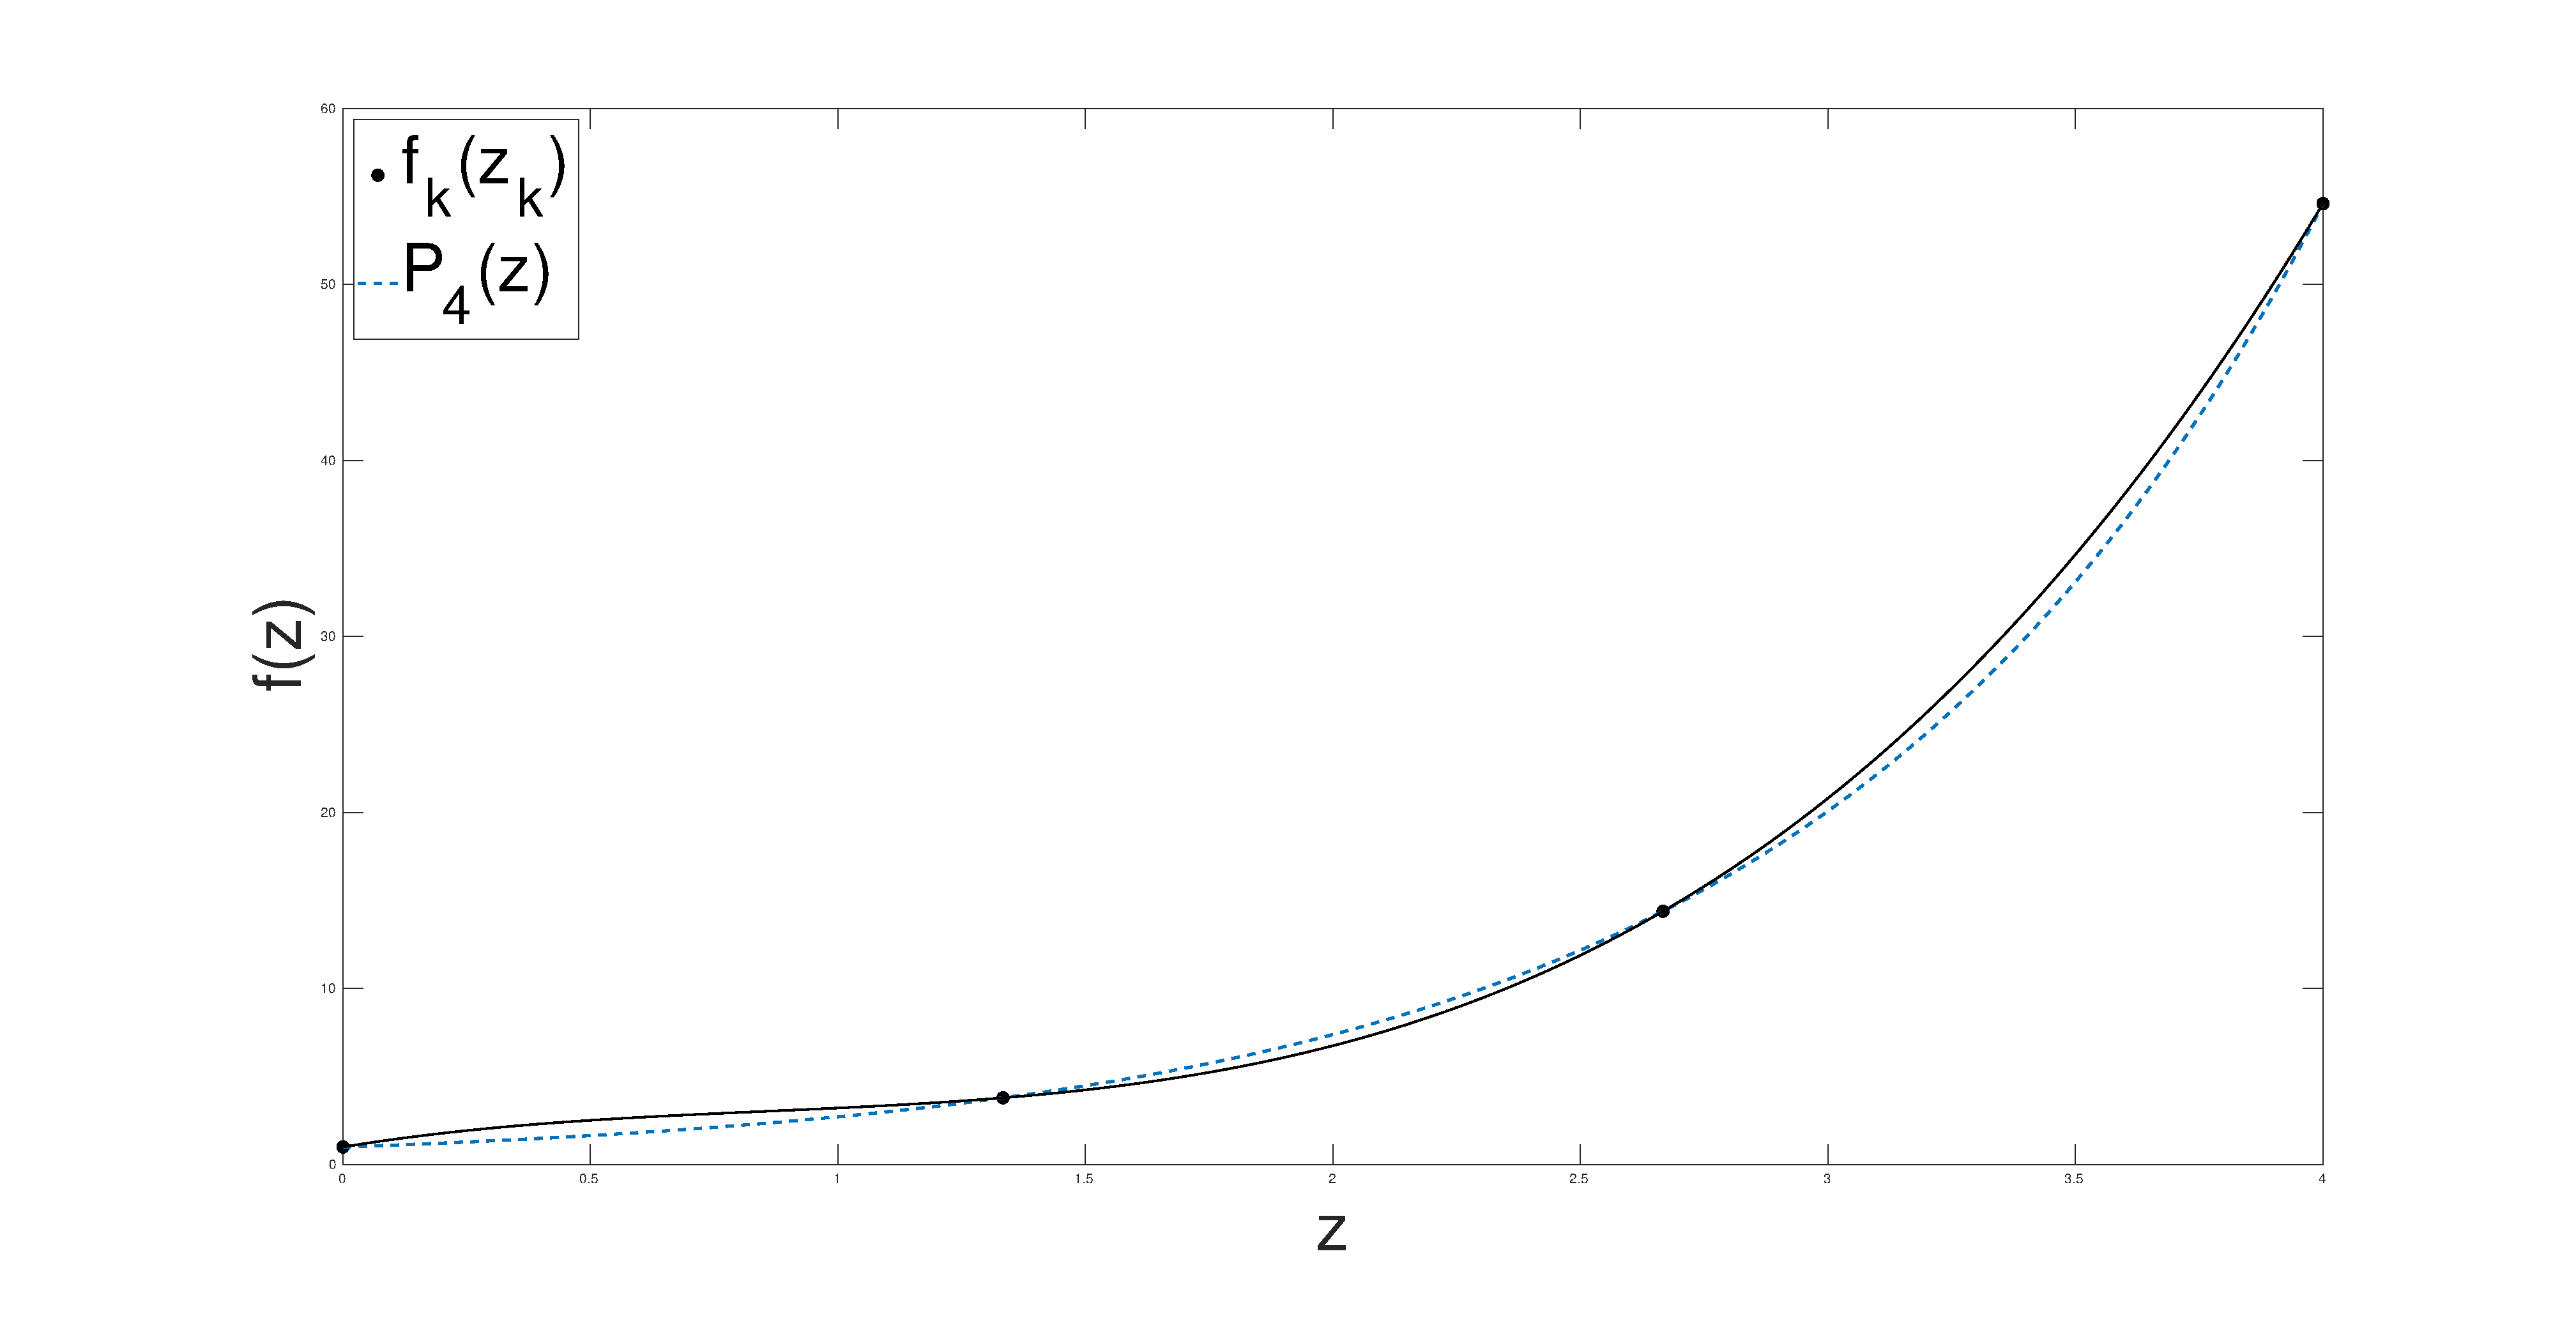
\includegraphics[trim={0 0cm 0 0cm},clip,width=1\textwidth]{FIGURES/lag_interp_plot2.eps}
					\caption{Depiction of $P_4(z)$}
		\end{figure}
		\end{center}
	\end{column}
	\begin{column}{0.5\textwidth}
		\vspace{1.5cm}
		\begin{center}
			\begin{itemize}
				\item $P_n(z) = \sum_{k=0}^{n} L_k(z)f_k $
				\vspace{0.5cm}
				\item $L_k(z) =  \prod_{j=0, j \neq k}^{n} \frac{z-z_j}{z_k-z_j}$
			\end{itemize}
		\end{center}
	\end{column}
\end{columns}
\end{frame}

\begin{frame}
\frametitle{Generate grid vertices}
\vspace{-1 cm}
\begin{columns}[onlytextwidth]
	\begin{column}{0.5\textwidth}
		\begin{center}
			\begin{figure}
				\includegraphics[trim={1cm 0cm 1cm 0cm},clip,width=1\textwidth]{FIGURES/Delaunay_Connected_PrismFaces.eps}
				\caption{2D grid vertices}
			\end{figure}
		\end{center}
	\end{column}
	\begin{column}{0.5\textwidth}
		\vspace{0 cm}
		\begin{center}
			\begin{itemize}
				\item Generate the vertex positions in poloidal plane
					\begin{itemize}
				\item set number of points per ring
				\item scale point distributions according to scaling functions for $s,~\vartheta$
			\end{itemize}
		\item Extrude vertex coordinates toroidally $(s,\vartheta, \varphi=0)\rightarrow (s,\vartheta, \varphi)$
		\end{itemize}
		\end{center}
	\end{column}
\end{columns}
\end{frame}

\begin{frame}
\frametitle{Mesh tetrahedra using Delaunay condition}
\vspace{-1.5cm}
\begin{columns}[onlytextwidth]
	\begin{column}{0.5\textwidth}
		\begin{center}
			\begin{figure}
				\includegraphics[trim={0cm 0cm 0cm 0cm},clip,width=0.9\textwidth]{FIGURES/Delaunay_Connected_PrismFaces.eps}
	\includegraphics[trim={0cm 0cm 0cm 0cm},clip,width=0.75\textwidth]{FIGURES/uvpq_Delaunay.eps}
			\end{figure}
		\end{center}
	\end{column}
	\begin{column}{0.5\textwidth}
		\vspace{0cm}
		\begin{center}
						\begin{itemize}
					\item index vertices to prism face of correct type \newline
					 $\rightarrow$ Delaunay condition 
				\end{itemize}
			\begin{figure}
	\includegraphics[trim={0cm 0cm 0cm 0cm},clip,width=1\textwidth]{FIGURES/2Prisms_comparison.eps}
	\caption{Prism types used for tetrahedra indexing}
\end{figure}
		\end{center}
	\end{column}
\end{columns}
\end{frame}

\begin{frame}
\frametitle{One compromise: there is a hole}
\vspace{-1cm}
%\begin{columns}[onlytextwidth]
%	\begin{column}{0.5\textwidth}
		\begin{center}
			\begin{figure}
				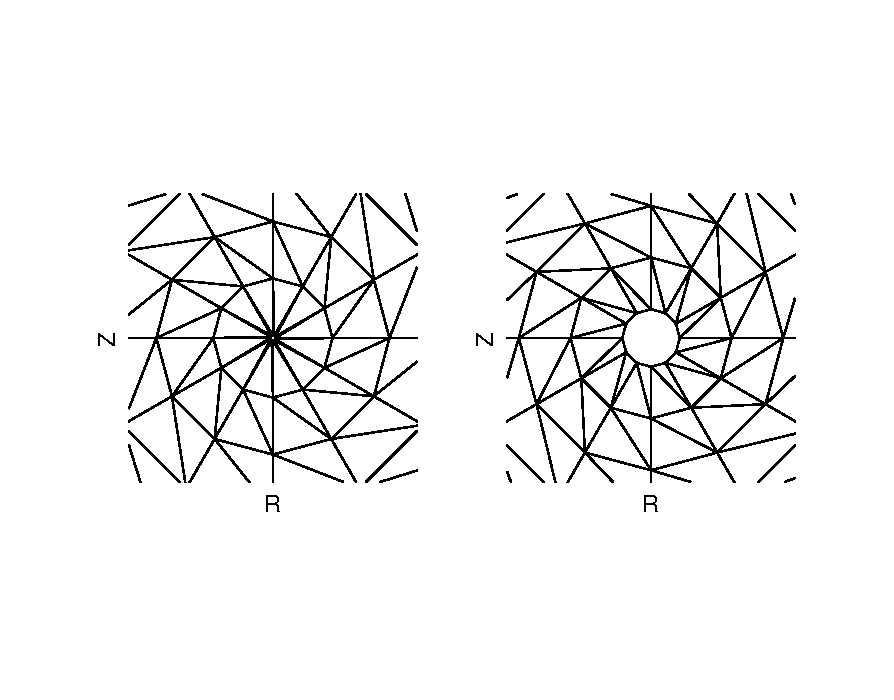
\includegraphics[trim={1cm 2cm 1cm 1cm},clip,width=1\textwidth]{FIGURES/Comparison_smin_annulus.eps}
				\caption{Center region of the grid with annulus}
			\end{figure}
		\end{center}
%	\end{column}
%	\begin{column}{0.5\textwidth}
%		\vspace{0cm}
%		\begin{center}
%			\begin{itemize}
%				\item
%			\end{itemize}
%		\end{center}
%	\end{column}
%\end{columns}
\end{frame}



\begin{frame}
\frametitle{Field aligned grid}
\vspace{-1cm}
%\begin{columns}[onlytextwidth]
%	\begin{column}{0.5\textwidth}
		\begin{center}
			\begin{figure}
				\includegraphics[trim={0cm 0cm 0cm 0cm},clip,width=1\textwidth]{FIGURES/Curvilinear_grid_and_tetrahedra.eps}
				\caption{Poloidal cross-section and grid elements of field aligned grid in real space}
			\end{figure}
		\end{center}
%	\end{column}
%	\begin{column}{0.5\textwidth}
%		\vspace{0cm}
%		\begin{center}
%			\begin{itemize}
%				\item
%			\end{itemize}
%		\end{center}
%	\end{column}
%\end{columns}
\end{frame}





\section{Numerical orbit calculation}


\begin{frame}
\frametitle{Computational approach}
\vspace{-0.5cm}
\begin{itemize}
	\item Piecewise-constant coefficients of 
	$$
	\frac{\rd z^i}{\rd \tau} = a^i_k z^k + b^i
	$$
	are discontinuous at cell boundaries. 
	\item Orbit intersections with tetrahedra faces must be computed exactly when integrating particle trajectories.
	
	\item The ODE set is numerically solved via \textbf{Runge-Kutta~4} in an iterative scheme.
	\item Iterative scheme uses \textbf{Newton's method} and a parabolic analytic estimation for the  initial step length.

\end{itemize}
\end{frame}

\begin{frame}
\frametitle{Analytical solution to ODE set}
\vspace{-1cm}
\begin{itemize}
	\item get homogeneous solution \newline
	\item get particular solution from variation of constants\newline
\end{itemize}

$\rightarrow x^i(\tau) =   \psi^i_l  \left(\bar{\psi}^l_k x^k_{(0)}e^{\lambda^l \tau} + \frac{\bar{\psi}^l_k D^k}{a-\lambda^l}(e^{a\tau}-e^{\lambda^l\tau}) + \right.$\\
\vspace{0.5cm}
\hspace{1.5cm}$\left. \frac{\bar{\psi}^l_k F^k}{2a-\lambda^l}(e^{2a\tau}-e^{\lambda^l\tau})-\frac{\bar{\psi}^l_k E^k}{\lambda^l}(1-e^{\lambda^l\tau}) \right)$
\end{frame}

\begin{frame}[noframenumbering]
\frametitle{Analytical solution to ODE set}
\vspace{-1cm}
\begin{itemize}
	\item get homogeneous solution \newline
	\item get particular solution from variation of constants\newline
\end{itemize}

$\rightarrow x^i(\tau) =   \psi^i_l  \left(\bar{\psi}^l_k x^k_{(0)}e^{\lambda^l \tau} + \frac{\bar{\psi}^l_k D^k}{a-\lambda^l}(e^{a\tau}-e^{\lambda^l\tau}) + \right.$\\
\vspace{0.5cm}
\hspace{1.5cm}$\left. \frac{\bar{\psi}^l_k F^k}{2a-\lambda^l}(e^{2a\tau}-e^{\lambda^l\tau})-\frac{\bar{\psi}^l_k E^k}{\lambda^l}(1-e^{\lambda^l\tau}) \right)$ \newline

Unfortunately, due to numerical inaccuracies and high computational cost, this is not useful!
\end{frame}

\begin{frame}
\frametitle{New approach: Taylor expansion of solution}
\vspace{0cm}
ODE set: $$\frac{\rd \textbf{z}}{\rd \tau} = \hat{\textbf{a}}\textbf{z} + \textbf{b}$$ \newline
\vspace{0cm}
Taylor series: $$\textbf{z}=\textbf{z}_0 + \sum\limits_{k=1}^\infty \frac{\tau^k}{k!}\hat{\textbf{a}}^{k-1}\cdot (\textbf{b} + \hat{ \textbf{a}} \cdot\textbf{z}_0)$$ \newline
$\rightarrow$ $RK4$ corresponds to fourth order expansion, thus the fifth order estimates the $RK4$-error!
\end{frame}

\begin{frame}
\frametitle{Evaluating the $RK4$ error - CCG}
\vspace{-1.5cm}
\begin{columns}[onlytextwidth]
	\begin{column}{0.5\textwidth}
		\begin{center}
			\begin{figure}
				\includegraphics[trim={9cm 0cm 10cm 0cm},clip,width=1\textwidth]{FIGURES/RK4_alpha555_cyl.pdf}
				\caption{$(N_R,N_\varphi,N_Z)= 5\times5\times5$}

			\end{figure}
		\end{center}
	\end{column}
	\begin{column}{0.5\textwidth}
		\vspace{0cm}
		\begin{center}
					\begin{figure}
					\includegraphics[trim={9cm 0cm 10cm 0cm},clip,width=1\textwidth]{FIGURES/RK4_alpha121212_cyl.pdf}
				\caption{$(N_R,N_\varphi,N_Z)= 12\times12\times12$}
							\end{figure}
%			\begin{itemize}
%				\item
%			\end{itemize}
		\end{center}
	\end{column}
\end{columns}
\end{frame}

\begin{frame}
\frametitle{Evaluating the $RK4$ error - FAG}
\vspace{-1.5cm}
\begin{columns}[onlytextwidth]
	\begin{column}{0.5\textwidth}
		\begin{center}
			\begin{figure}
				\includegraphics[trim={9cm 0cm 10cm 0cm},clip,width=1\textwidth]{FIGURES/RK4_alpha555_SFC.pdf}
				\caption{$(N_s,N_\vartheta,N_\varphi)= 5\times5\times5$}
				
			\end{figure}
		\end{center}
	\end{column}
	\begin{column}{0.5\textwidth}
		\vspace{0cm}
		\begin{center}
			\begin{figure}
				\includegraphics[trim={9cm 0cm 10cm 0cm},clip,width=1\textwidth]{FIGURES/RK4_alpha121212_SFC.pdf}
				\caption{$(N_s,N_\vartheta,N_\varphi)= 12\times12\times12$}
			\end{figure}
			%			\begin{itemize}
			%				\item
			%			\end{itemize}
		\end{center}
	\end{column}
\end{columns}
\end{frame}

%\begin{frame}
%\frametitle{}
%\vspace{0cm}
%\begin{columns}[onlytextwidth]
%	\begin{column}{0.5\textwidth}
%		\begin{center}
%			\begin{figure}
%				\includegraphics[trim={0cm 0cm 0cm 0cm},clip,width=1\textwidth]{FIGURES/}
%				\caption{}
%			\end{figure}
%		\end{center}
%	\end{column}
%	\begin{column}{0.5\textwidth}
%		\vspace{0cm}
%		\begin{center}
%			\begin{itemize}
%				\item
%			\end{itemize}
%		\end{center}
%	\end{column}
%\end{columns}
%\end{frame}


%%\begin{frame}
%%\frametitle{Error of the RK~4 method}
%%\vspace{-0.5cm}
%%\begin{itemize}
%%	\item The relative integration error of a single step between cell boundaries strongly \textbf{scales %with the Larmor radius $\rho$}.
%%	
%%	\item The error is in the order of
%%	\be{RK4estimation}
%%	\frac{\delta R(\Delta\tau)}{a} \sim \frac{\rho^3}{q^4 R^3} \Delta \varphi^5,
%%	\ee
%%	with $R$, $a$, $q$ and $\Delta\varphi$ denoting major radius, plasma radius, safety factor and %toroidal cell length.
%%	
%%	\item 
%%	The \textbf{error of the RK4 method} can be brought \textbf{below computer accuracy}.
%%\end{itemize}
%%\end{frame}

\begin{frame}
\frametitle{Poincare plots of guiding center orbits}
\note{Alles erklaeren}
\vspace{-1.1cm}
%\hspace{-7cm}
\begin{figure}
	\hspace*{-0.9cm}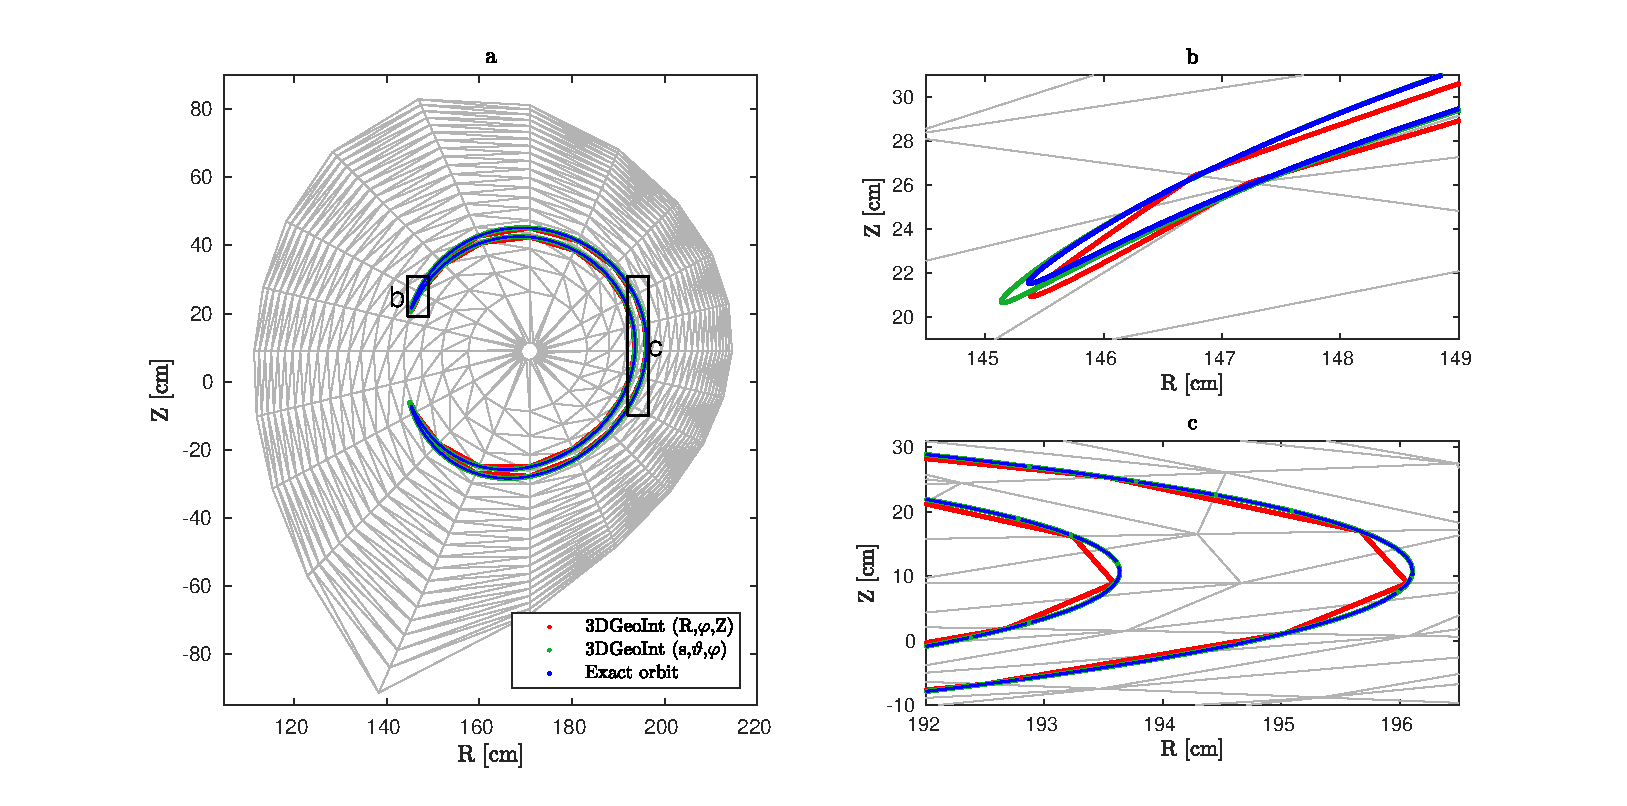
\includegraphics[width=1.0\textwidth]{FIGURES/orbit_plot.eps}
\end{figure}
\begin{itemize}
	\vspace*{-0.5cm}
\item Geometric integration: Not exact orbit shape.
\item Axisymmetic (2D): Canonical toroidal angular momentum is preserved.
\end{itemize}
\end{frame}

\begin{frame}
\frametitle{Axisymmetric noise of electrostatic and vector potential}
\vspace{-0.4cm}
%\hspace{-7cm}
\begin{figure}
	\hspace*{-1.05cm}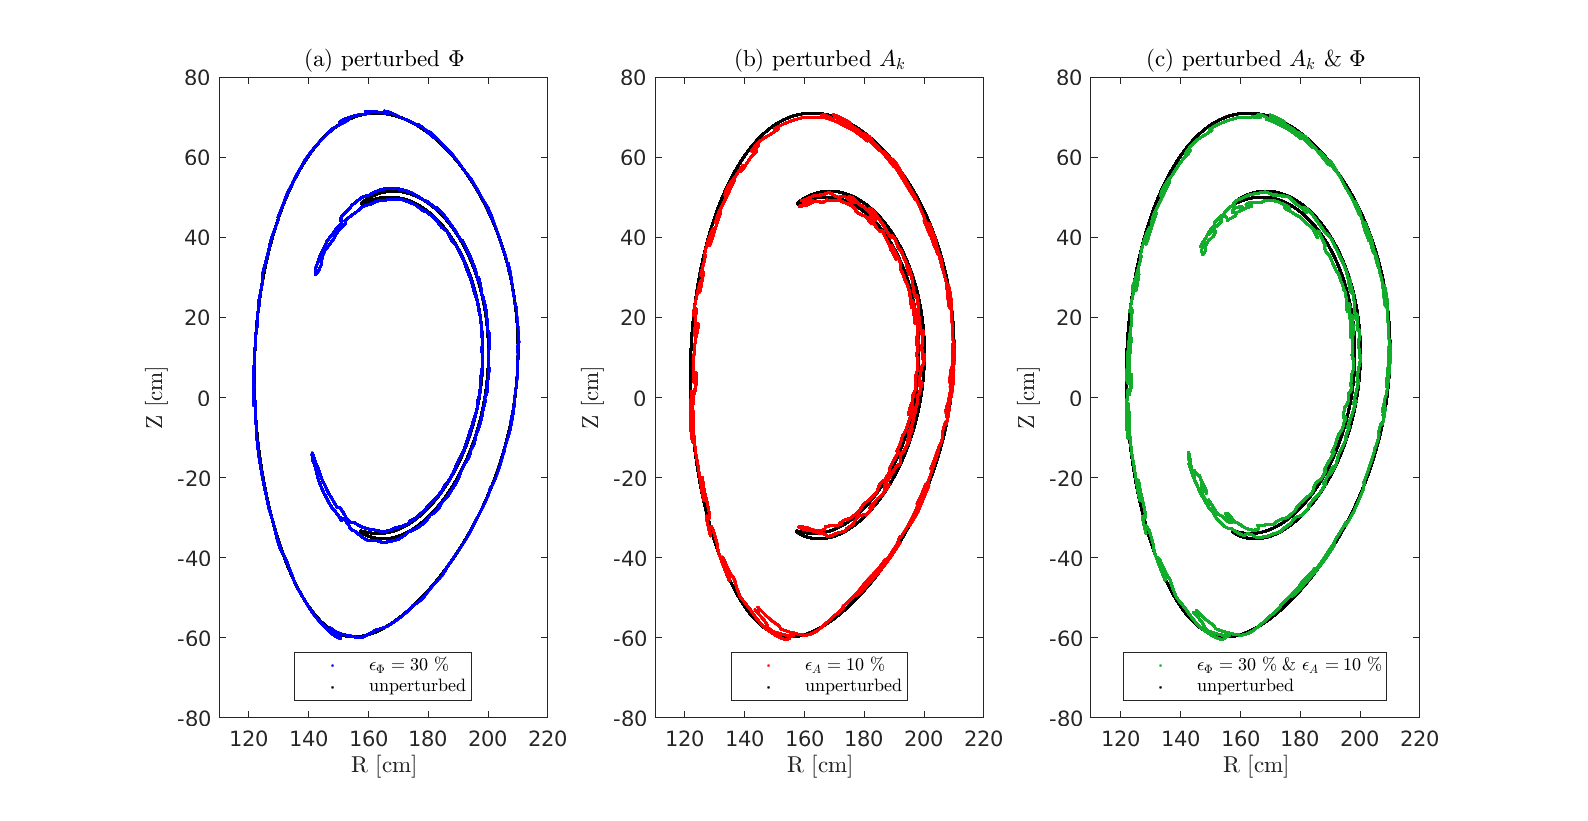
\includegraphics[width=1.0\textwidth]{FIGURES/axissymetric_noise.eps}
\end{figure}
\begin{itemize}
	\vspace*{-0.6cm}
	\item Similar orbit shape (compared to unperturbed orbit)
	\item Canonical toroidal angular momentum is preserved.
\end{itemize}
\end{frame}

%\section{Artifact: Numerical diffusion}

%\begin{frame}
%\frametitle{Artifact: Numerical field line diffusion}
%\vspace{-0.5cm}
%\begin{itemize}
%\item
%Due to the linearization of fields for 3D configurations, \textbf{KAM surfaces do not exist anymore}. \\
%$\rightarrow$ \textbf{ergodic passing particle orbit}
%\item This behaviour is\textbf{ diffusive} and its
%variance can be described by a field line diffusion coefficient $D_M^{ss}$ as
%$\left\langle \delta s^2\right\rangle=2 D_M^{ss} N$ where $N$ is the number of toroidal orbit turns.
%\item \textbf{Strong inverse scaling} of \textbf{$D_M^{ss}$ with poloidal $N_\vartheta$ and toroidal $N_\varphi$ grid sizes}, which roughly agrees with 
%\be{quasilinear_diffco}
%D^{ss}_M = \frac{2 \pi^2}{3} \left( \frac{\psi_{\text{pol}} \epsilon_M }{\psi_{\text{tor}}^a}\right)^2 \frac{q^4 m_0^2 n_0^2 
%	\left(m_0 N_\vartheta + n_0 N_\varphi \right)^2}{N_\vartheta^2 N_\varphi^2 \left( q N_\varphi-N_\vartheta\right)^2}.
%\ee
%\vspace{-1cm}
%\tiny{(quasilinear theory)}
%\vspace{1cm}
%\end{itemize}
%\end{frame}


%\begin{frame}
%\frametitle{Artifact: Numerical field line diffusion}
%\vspace{-1.4cm}
%%\hspace{-7cm}
%\begin{figure}
%\hspace*{-1.4cm}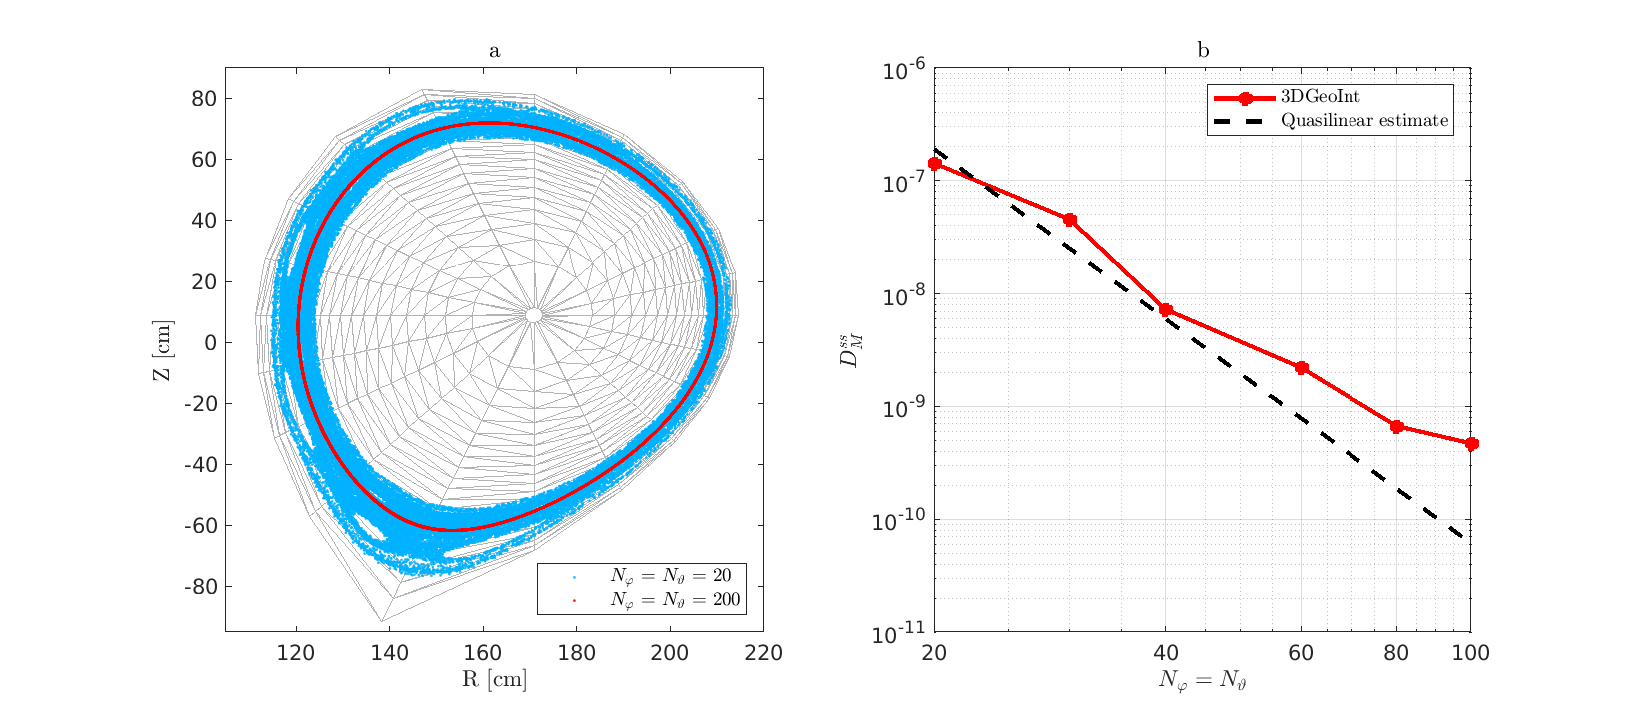
\includegraphics[width=1.25\textwidth]{FIGURES/diffusion.eps}
%\end{figure}
%\end{frame}



%\begin{frame}
%\frametitle{Artifact: Numerical field line diffusion II}
%\vspace{-0.5cm}
%\begin{itemize}
%	\item Numerical diffusion can be put \textbf{below the level of classical electron diffusion}
%	using a mild \textbf{grid refinement}.
%	\item
%	When tracing orbits in a \textbf{VMEC stellarator field} numerical diffusion is effectively \textbf{minimized by using symmetry flux coordinates}.
%	\begin{itemize}
%	\item Numerical diffusion results only from the FLR effects which lead roughly to the same
%	order of perturbations as in weakly perturbed tokamaks, $\varepsilon_M \sim \rho/a$.
%\end{itemize} 
%	\end{itemize}
%\end{frame}
%
%\begin{frame}
%\frametitle{Turning artifact into feature:}
%\vspace*{-0.5cm}
%\textit{\textbf{Numerical diffusion for anomalous transport modelling:}}
%\begin{itemize}
%	\item 3D noise in ($\vec{A}$,$\Phi$) leads to artificial diffusion.
%	\item Use this diffusion as an additional transport mechanism
%	to model anomalous transport.
%	\item The resulting orbits are physically consistent .
%	\item Adjust amplitude of the noise to reproduce phenomenological transport coefficient.
%\end{itemize}
%
%\end{frame}
%

%\section{Generating the field aligned grid}

%\begin{frame}
%\frametitle{3D field aligned grid: tetrahedral cells}
%\vspace{-1.7cm}
%%\hspace{-7cm}
%	\begin{figure}
%		\hspace*{-1.65cm}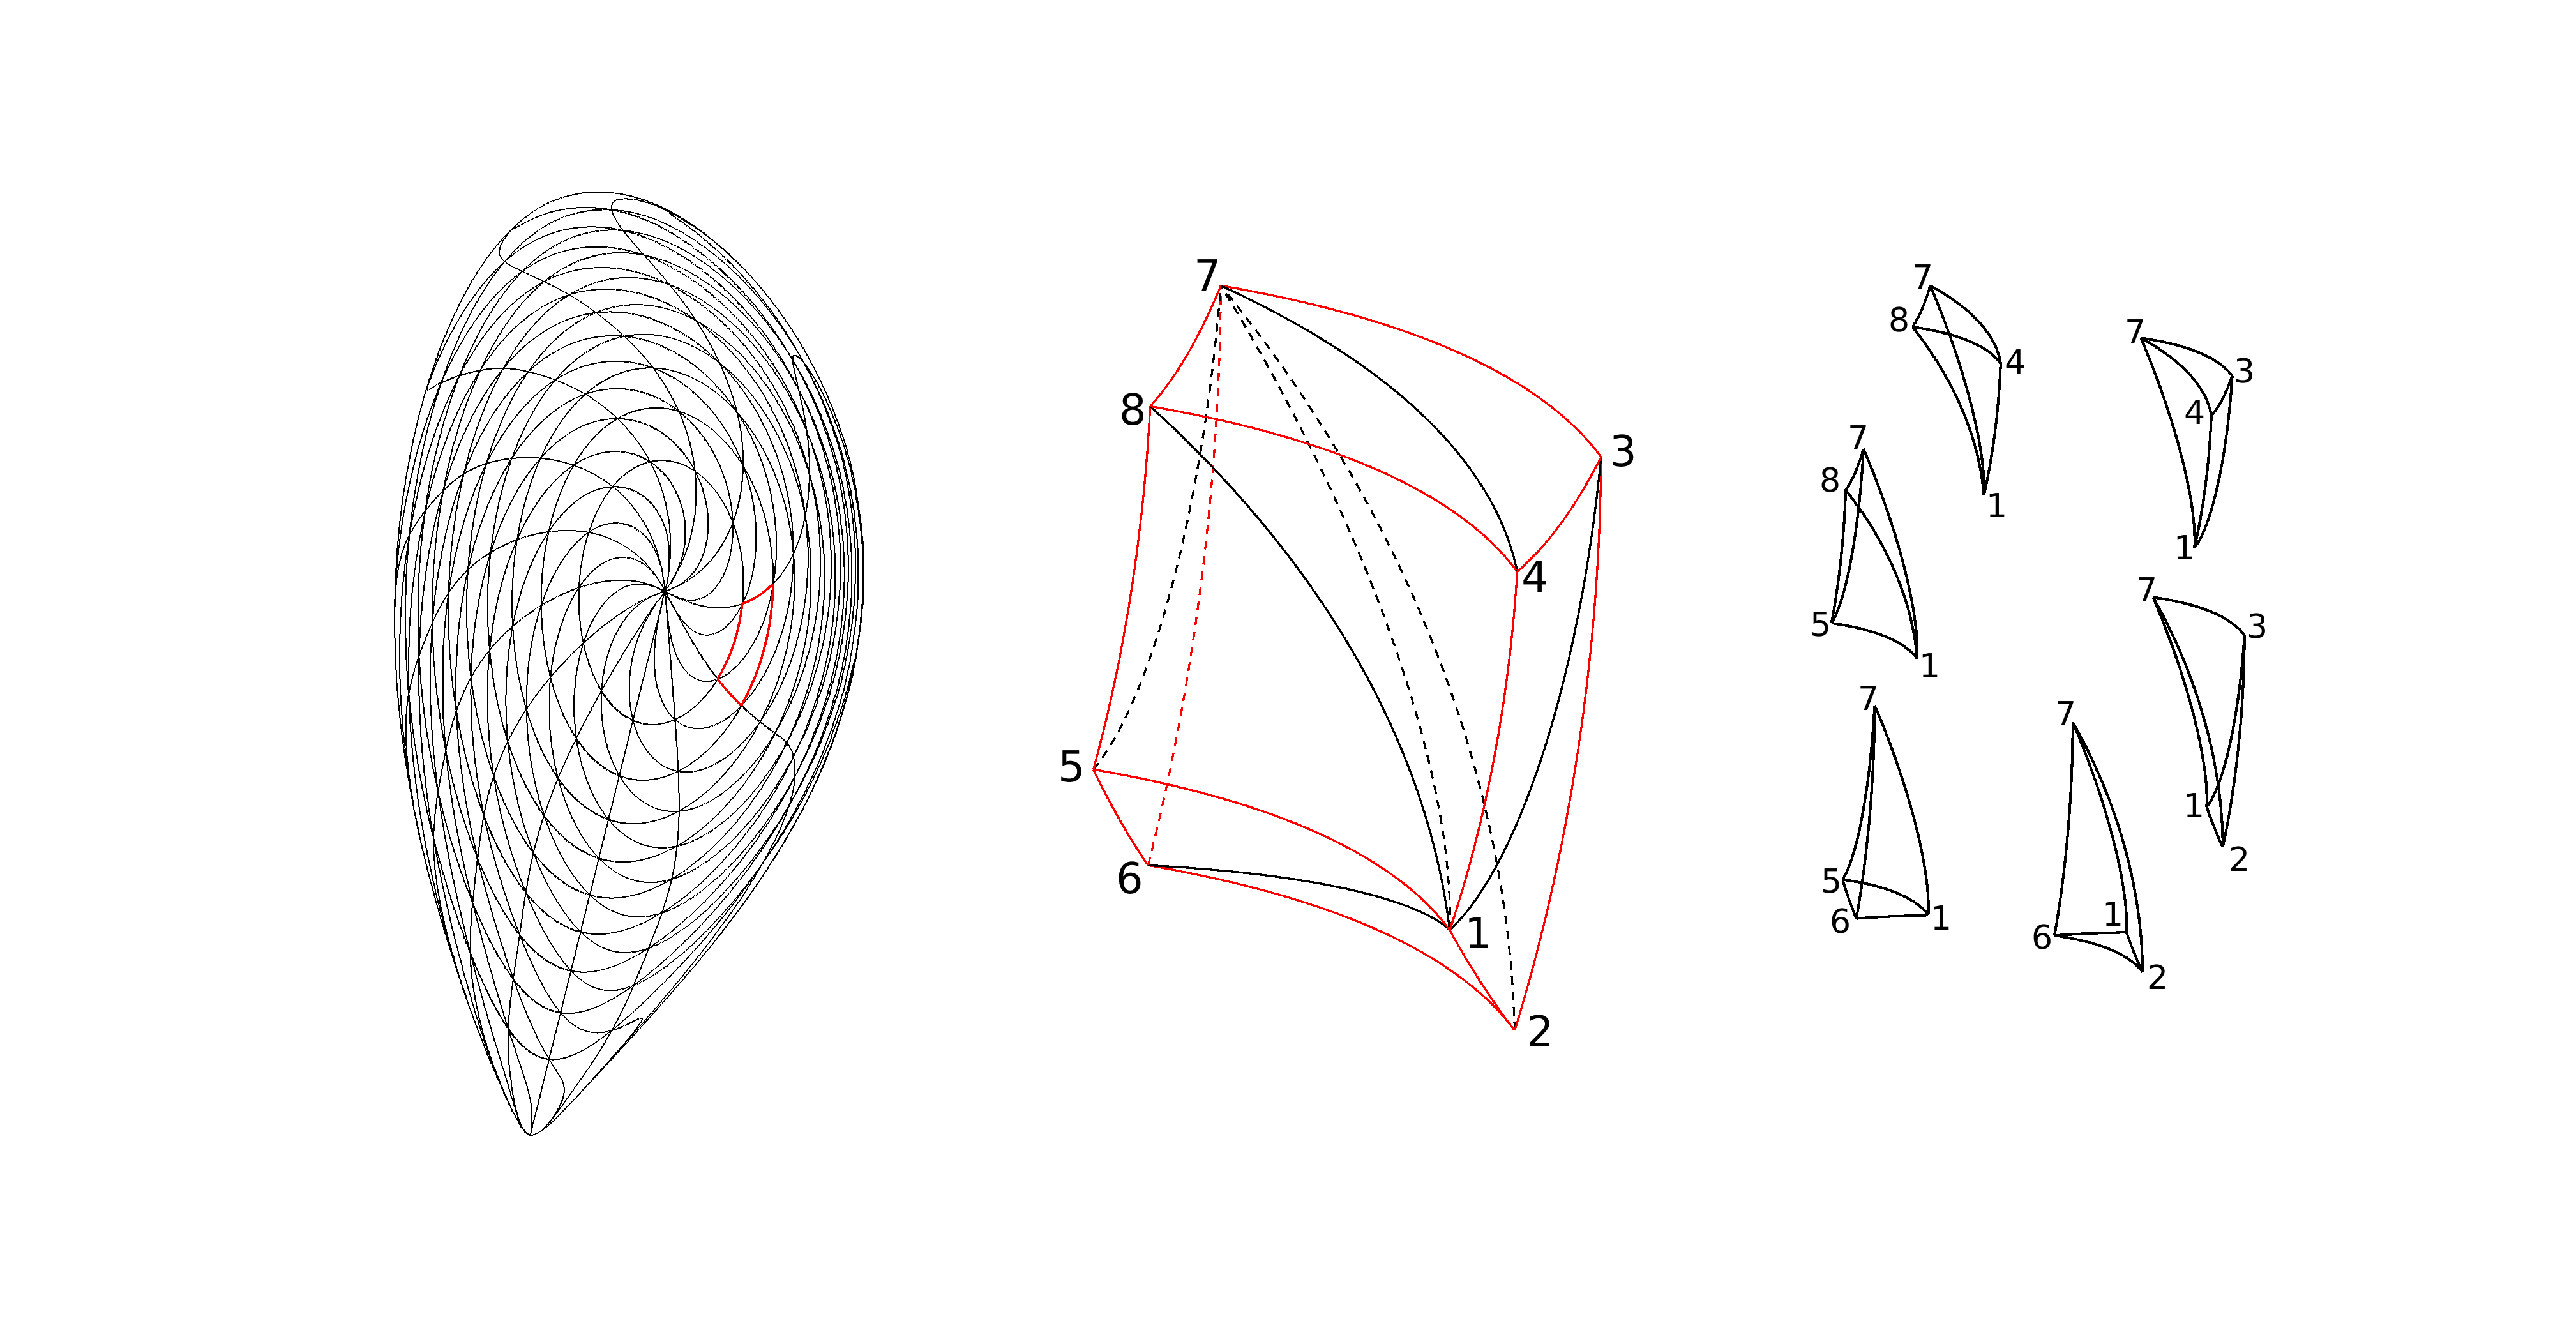
\includegraphics[width=1.25\textwidth]{FIGURES/curvilinear_grid.eps}
%	\end{figure}
%
%\end{frame}

\section{Application: Mono-energetic radial transport coefficient}


\begin{frame}
\frametitle{Application: Mono-energetic radial transport coefficient}
\vspace{-0.5cm}
\begin{itemize}
	\item Mono-energetic radial transport coefficient as a function of collisionality is evaluated with the Monte Carlo method.
	\item Collisions are realized by pitch angle scattering (Lorentz scattering operator).\\
	\be{}
	\frac{\partial f}{\partial t} = \frac{1}{s \left(\psi \right)} \frac{\partial}{\partial \psi}s D 	\frac{\partial f}{\partial \psi} 
	\ee
	\be{}
	D = D(E,\psi) = \langle \frac{1}{2t} \left( \psi  \left(t\right) - \psi \left( t_0 \right) \right)^2 \rangle
	\ee
\end{itemize}
\end{frame}



\begin{frame}
\frametitle{Radial Transport in HYDRA (stellarator)}
\vspace{-1.2cm}
%\hspace{-7cm}
\hspace*{0.1cm}
\begin{columns}[t]
	\begin{column}{0.8\textwidth}
		\begin{figure}
			\vspace*{-1.05cm}
\hspace*{-0.5cm}\includegraphics[width=1\textwidth]{FIGURES/transport_coefficient_electrons_dions.eps}

\end{figure}
\end{column}
\hspace*{-1cm}
\begin{column}{0.2\textwidth}
	\vspace*{0.8cm}
	\bea*{} 
		\nu^{\ast} &=& \frac{R_0 \nu_c}{\iota v} \nonumber \\
		\quad \nonumber \\ 
		v_E^{\ast} &=& \frac{E_r}{v B_0} \nonumber
	\eea
	
	\end{column}
\end{columns}
Mono-energetic radial diffusion coefficient,\newline
$E_{kin}=$ 3 keV, $s_0 = 0.6$
\end{frame}


\section{Conclusion}
\begin{frame}
\frametitle{Conclusion}
\vspace*{-0.5cm}
%\textit{\textbf{Advantages:}}\\
\begin{itemize}
\item Physically correct long time orbit dynamics
\item Particle coordinates and velocities are implicitly given at cell boundaries.
\item Low sensitivity to noise in electromagnetic fields
\item Computational efficiency
\end{itemize}
%\textit{\textbf{Limitations:}}
%\begin{itemize}
%\item Artificial numerical diffusion is induced by piecewise linear field quantities.
%\end{itemize}
\end{frame}

\section{Conclusion}



\section{ }
 \begin{frame}
% \frametitle{Motivation for planned\\ impurity transport modelling (2)}
% \vspace{-1mm}
% \includegraphics[width=\textwidth,height=0.8\textheight]{AUG32169_profiles}
% \begin{picture}(0,0)
% \put(0,190) {\tiny \turnbox{-90}{P. Piovesan et al, Plasma Phys. Control. Fusion 59 (2017) 014027}}
% \end{picture}
\vspace*{2.5cm}
\centerline{\huge Thank you for your attention!}
 \end{frame}



%%%%%%%%%%%%%%%%%%%%%%%%%%%%%%%%%%%%%%%%%%%%%%%%%%%%%%%%%%%%%%%%%%%%%%%%%%%%
\end{document}
%%%%%%%%%%%%%%%%%%%%%%%%%%%%%%%%%%%%%%%%%%%%%%%%%%%%%%%%%%%%%%%%%%%%%%%%%%%%

%% EOF
